\documentclass[UTF8, 12pt]{ctexart}
\usepackage{color}
% 颜色
\definecolor{orange}{RGB}{255,127,0} 
\usepackage{amssymb}
% 因为所以
\usepackage{amsmath}
% 数学公式
\setcounter{tocdepth}{5}
\setcounter{secnumdepth}{5}
% 设置四级目录
\usepackage{geometry}
\geometry{papersize={21cm,29.7cm}}
\geometry{left=3.18cm,right=3.18cm,top=2.54cm,bottom=2.54cm}
% 设置页边距
\usepackage{indentfirst}
\setlength{\parindent}{2.45em}
% 设置首行缩进
\usepackage{setspace}
\renewcommand{\baselinestretch}{1.5}
% 设置行距
\usepackage{tikz}
% 绘图
\usetikzlibrary{positioning}
% 为了实现相对位置的设定
\usepackage{xcolor}
% 为了实现不同的颜色
\author{Didnelpsun}
\title{考研数学准备}
\begin{document}
\maketitle
\thispagestyle{empty}
\tableofcontents
\thispagestyle{empty}
\newpage
\pagestyle{plain}
\setcounter{page}{1}
\section{函数的概念与特性}
\subsection{函数}
\begin{itemize}
    \item 函数即$y=f(x),x\in D$,x为自变量,y为因变量,D为定义域
    \item 一个x对应一个y,一个y可能对应多个x。
\end{itemize}
\subsection{反函数}
$y=f(x)$,定义域为$D$,值域为$R$,若对于每一个$y\in R$,必然存在$x\in D$使$y=f(x)$成立,则可以定义一个新函数$x=\psi(y)$,这个函数就是$y=f(x)$的\textbf{反函数},一般记作$x=f^{-1}(y)$,其定义域为$R$,值域为$D$,对于反函数,原来的函数称为\textbf{直接函数}。
\begin{enumerate}
    \item \textcolor{red}{严格单调}函数必然有反函数,即函数导数恒正或恒负必然有反函数。
    \item $x=f^{-1}(y)$与$y=f(x)$在同一坐标系中完全重合。
    \item $y=f^{-1}(x)$与$y=f(x)$关于$y=x$对称。
    \item $f[f^{-1}(x)]$或$f[\psi(x)]$变为x,称为湮灭。
\end{enumerate}
\subsection{复合函数}
设$y=f(u)$的定义域为$D_1$,函数$u=g(x)$在$D$上有定义且$g(D)\in D$,则由$y=f[g(x)],x\in D$确定的函数称为由函数$u=g(x)$和函数$y=f(u)$构成的复合函数,定义域为D,u为中间变量。

\textbf{例题1:}设$f(x)=x^2$,$f[\psi(x)]=-x^2+2x+3$,且$\psi(x)\geqslant 0$,求$\psi(x)$以及定义域与值域。

广义化:$\because f(x)=x^2$,$\therefore f[\psi(x)]=\psi^2(x)=-x^2+2x+3$

又$\because\psi(x)\geqslant 0$, $\therefore\sqrt{\psi^2(x)}=\sqrt{-x^2+2x+3}=\psi(x)\geqslant 0$

$\therefore x\in[-1,3]$

$\therefore\frac{\rm{d}\psi(x)}{\rm{d}x}=(-x^2+2x+3)'=-2x+2=0$

$\therefore x=1$,驻点为1

又$\because(-x^2+2x+3)''=-2<0$

$\therefore$驻点为1时为最大值点,最大值为$\psi(1)=2$

又$\because\psi(-1)=\psi(3)=0$,$\therefore$最小值为0

$\therefore\psi(x)\in[0,2]$

\textcolor{orange}{注意}:$\sqrt{-x^2+2x+3}$为什么最值与$-x^2+2x+3$一致?

\textbf{例题2:}求函数$y=f(x)=\ln(x+\sqrt{x^2+1})$的反函数$f^{-1}(x)$的表达式及其定义域

首先研究$f(x)$本身,因为$\ln(x)$的定义域必然要求大于0,而任意实数x都有下面不等式成立:

$x+\sqrt{x^2+1}>x+\vert x\vert \geqslant 0$,所以$x\in R$。

而研究其奇偶性:

$f(-x)=\ln(-x+\sqrt{x^2+1})=\ln(\frac{1}{\sqrt{x^2+1}+x})=-\ln(x+\sqrt{x^2+1})=-f(x)$

所以该函数为奇函数。

对其求单调性,即通过链式法则求导:

$\frac{\rm{d}y}{\rm{d}x}=\frac{1}{x+\sqrt{x^2+1}}\cdot (1+\frac{2x}{2\sqrt{x^2+1}})=\frac{1}{\sqrt{x^2+1}}>0$

所以该函数严格单调增。

然后求$y$的反函数:

$$
    \begin{aligned}
        \because y & =\ln(x+\sqrt{x^2+1})     \\
        e^y        & =e^{\ln(x+\sqrt{x^2+1})} \\
                   & =x+\sqrt{x^2+1}
    \end{aligned}
$$

$$
    \begin{aligned}
        \because -y & =-\ln(x+\sqrt{x^2+1})          \\
                    & =\ln(\frac{1}{x+\sqrt{x^2+1}}) \\
                    & =\ln(\sqrt{x^2+1}-x)           \\
        e^{-y}      & =\sqrt{x^2+1}-x
    \end{aligned}
$$

$$
    \begin{aligned}
        \therefore e^y-e^{-y} & =2x                   \\
        x                     & =\frac{e^y-e^{-y}}{2}
    \end{aligned}
$$

解出了用x表示y的函数表达$x=f^{-1}(y)$,即反函数,则$f^{-1}(x)=\frac{e^x-e^{-x}}{2}$

这种曲线为一种常见曲线:

\begin{itemize}
    \item $\frac{e^x-e^{-x}}{2}$:双曲正弦。
    \item $\frac{e^x+e^{-x}}{2}$:双曲余弦。(为一种悬链线)
    \item $\ln(x+\sqrt{x^2+1})$:反双曲正弦。
    \item $\ln(x+\sqrt{x^2-1})$:反双曲余弦。
\end{itemize}

\textbf{例题3:}设$
    f(x)=\left\{
    \begin{array}{rcl}
        \ln\sqrt{x}, &  & x\geqslant 1 \\
        2x-1,        &  & x< 1
    \end{array}
    \right.
$,求$f[f(x)]$

首先广义化:$
    f[f(x)]=\left\{
    \begin{array}{rcl}
        \ln\sqrt{f(x)}, &  & f(x)\geqslant 1 \\
        2f(x)-1,        &  & x<1
    \end{array}
    \right.
$

然后画图:\bigskip

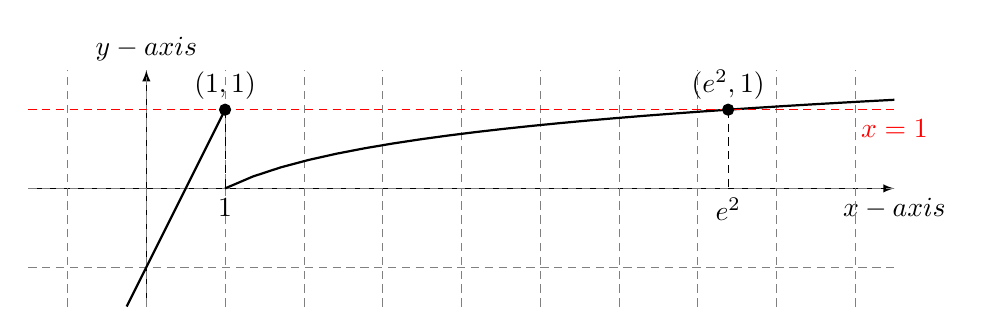
\begin{tikzpicture}[domain=-1:9.5]
    \draw[-latex](-1.5,0) -- (9.5,0) node[below]{$x-axis$};
    \draw[-latex](0,-1.5) -- (0, 1.5) node[above]{$y-axis$};
    \draw[very thin, gray, densely dashed](-1.5,1.5)grid(9.5,-1.5);
    \draw [black, thick](-0.25,-1.5) -- (1,1);
    \draw[black, thick,domain=1:9.5] plot (\x, {ln(sqrt(\x))});
    \draw [red, densely dashed](-1.5,1) -- (9.5,1) node[below]{$x=1$};
    \filldraw [black] (1,1) circle (2pt) node[above]{$(1,1)$};
    \filldraw [black] (e^2,1) circle (2pt) node[above]{$(e^2,1)$};
    \draw[densely dashed](1,1) -- (1, 0) node[below]{$1$};
    \draw[densely dashed](e^2,1) -- (e^2,0) node[below]{$e^2$};
\end{tikzpicture}

所以将定义域分为三段:$[-\infty ,1],[1,e^2],[e^2, +\infty]$,然后根据不同定义域对应的不同函数再代回$f[f(x)]$:

$$
    f[f(x)]=\left\{
    \begin{array}{rcl}
        \ln\sqrt{\ln\sqrt{x}}, &  & x\geqslant e^2   \\
        \ln x-2,               &  & 1\geqslant x<e^2 \\
        4x-3,                  &  & x<1
    \end{array}
    \right.
$$

\subsection{有界性}

函数指明定义域区间才能讨论函数是否有界。

证明有界性:函数$f(x)$的定义域$D$,数集$I\in D$,如果存在某正数$M$,对于任一$x\in I$,有$\vert f(x)\vert\leqslant M$,则$f(x)$在$I$上有界,否则无界。

\subsection{单调性}

$\begin{matrix}
        \frac{\rm{d}y}{\rm{d}x}>0 & \Rightarrow & (x_1-x_2)[f(x_1)-f(x_2)]>0 & \Rightarrow & f(x)\nearrow  \\
        \frac{\rm{d}y}{\rm{d}x}<0 & \Rightarrow & (x_1-x_2)[f(x_1)-f(x_2)]<0 & \Rightarrow &f(x)\searrow
    \end{matrix}
$

\subsection{奇偶性}

\begin{enumerate}
    \item 奇函数:关于原点对称,$f(-x)=-f(x)$。
    \item 偶函数:关于y轴对称,$f(-x)=f(x)$。
    \item 对于定义在$[-l,l]$上的任意函数$f(x)$,$F_1(x)=f(x)-f(-x)$必为奇函数,$F_2(x)=f(x)+f(-x)$必为偶函数。可以参考上面所说的双曲正弦与双曲余弦函数。
    \item 若奇函数在0处有定义,那么$f(0)=0$。
    \item 若偶函数在0处存在导数,那么$f'(0)=0$,即x=0,曲线必然水平,即导数为0。
    \item 若函数$y=f(x)$的函数关于直线$x=T$对称的充分必要条件是$f(x)=f(2T-x)/f(x+T)=f(x-T)$。(令$T-x=t$进行换元计算得到)
\end{enumerate}

\textcolor{orange}{注意}:0和1处的函数定义应该注意。

如当a为0时:$f(b)-f(a)=f'(\xi )(b-a)=f(b)=bf'(\xi)$

如$f(x)>xf(1)$变形为$\frac{f(x)}{x}>f(1)$,辅助函数$F(x)=\frac{f(x)}{x}$

所以加减法警惕0,乘除法警惕1。

\subsection{周期性}

$f(x+T)=f(x)$,其中T为周期。 \bigskip

\textcolor{red}{重要结论:}

\begin{enumerate}
    \item 若$f(x)$为可导的偶函数,则$f'(x)$为奇函数。(1.4.1.1)
    \item 若$f(x)$为可导的奇函数,则$f'(x)$为偶函数。(1.4.1.2)
    \item 若$f(x)$为周期函数,则$f'(x)$也为周期函数且周期不变。(1.4.2)
    \item 连续的奇函数的一切原函数都是偶函数。(1.8.6)
    \item 连续的偶函数的原函数中仅有一个原函数是奇函数。(1.8.6)
    \item 若连续函数$f(x)$以T为周期且$\int_{0}^{T}f(x)\rm{d}x=0$,则$f(x)$的一切原函数也以T为周期。(1.8.8)
    \item 若$f(x)$在有限区间$(a,b)$中可导且$f'(x)$有界,则$f(x)$在$(a,b)$有界。(某一函数在固定区间内变化率是有界的,则变化范围是有界的)
\end{enumerate}

\section{函数的图像}
\subsection{直角坐标系图像}
\subsubsection{常见图像}
\paragraph{基本初等函数与初等函数} \leavevmode \bigskip

基本初等函数包括:常数函数、幂函数、指数函数、对数函数、三角函数、反三角函数。

\subparagraph{常数函数} \leavevmode \bigskip

$y=A$,A为常数,图像平行于x轴:

\begin{tikzpicture}[domain=-1:5]
    \draw[-latex](-1,0) -- (5,0) node[below]{$x-axis$};
    \draw[-latex](0,-0.5) -- (0, 1.5) node[above]{$y-axis$};
    \draw[black, thick](-1,1) -- (5,1) node[below]{$y=A$};
\end{tikzpicture}

\subparagraph{幂函数} \leavevmode \bigskip

$y=x^{\mu}$,$\mu$为实数,当$x>0$,$y=x^{\mu}$都有定义:

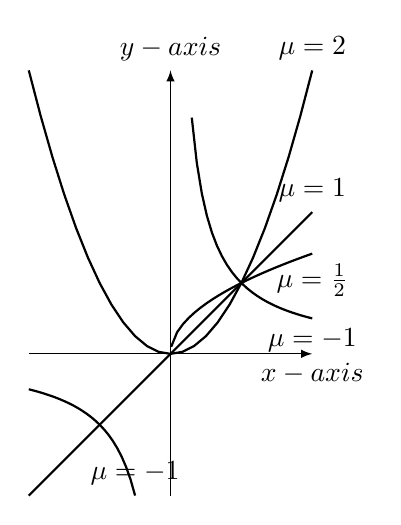
\begin{tikzpicture}[scale=0.9]
    \draw[-latex](-2,0) -- (2,0) node[below]{$x-axis$};
    \draw[-latex](0,-2) -- (0,4) node[above]{$y-axis$};
    \draw[black, thick, domain=0.3:2] plot (\x,1/\x) node[below]{$\mu =-1$};
    \draw[black, thick, domain=-2:-0.5] plot (\x,1/\x) node[above]{$\mu =-1$};
    \draw[black, thick, domain=0.01:2] plot (\x, {sqrt(\x)}) node[below]{$\mu =\frac{1}{2}$};
    \draw[black, thick, domain=-2:2] plot (\x,\x) node[above]{$\mu =1$};
    \draw[black, thick, domain=-2:2] plot (\x, {\x*\x}) node[above]{$\mu =2$};
\end{tikzpicture}

所以对于幂函数,可以根据不同幂下相同单调性来研究最值:

\begin{enumerate}
    \item $\sqrt{u},\sqrt[3]{u}$可以使用$u$来研究。
    \item $\vert u\vert$可以使用$u^2$来研究。
    \item $\frac{1}{u},u>0$可以使用$u$来研究,但是最值相反。
    \item $u_1u_2...u_n$可以使用$\sum_{i=1}^{n}\ln u_i$来研究。
\end{enumerate}

\subparagraph{指数函数} \leavevmode \bigskip

$y=a^x(a>0,a\neq 1)$:

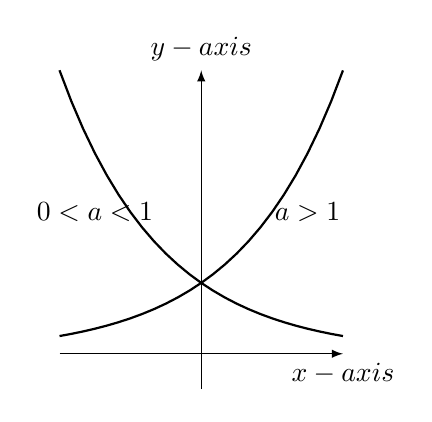
\begin{tikzpicture}[scale=0.9]
    \draw[-latex](-2,0) -- (2,0) node[below]{$x-axis$};
    \draw[-latex](0,-0.5) -- (0,4) node[above]{$y-axis$};
    \draw[black, thick, domain=-2:2] plot (\x,{pow(1/2,\x)}) node at (-1.5,2){$0<a<1$};
    \draw[black, thick, domain=-2:2] plot (\x,{pow(2,\x)}) node at (1.5,2){$a>1$};
\end{tikzpicture}

指数函数具有如下性质:

\begin{enumerate}
    \item 特殊函数值:$a^0=1$。
    \item 定义域:$(-\infty, +\infty)$,值域:$(0,+\infty)$。
    \item 单调性:$a>1$,$y=a^x$单调增,$0<a<1$,$y=a^x$单调减。
    \item 常用指数函数:$y=e^x$。
    \item 极限:$\lim_{x\to -\infty}e^x=0$,$\lim_{x\to +\infty}e^x=+\infty$。
\end{enumerate}

\subparagraph{对数函数} \leavevmode \bigskip

$y=log_ax(a>0,a\neq 1)$为$y=a^x$的反函数:

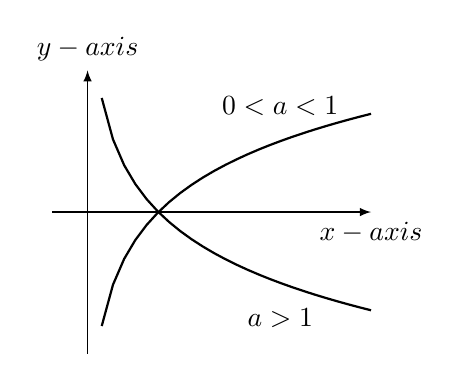
\begin{tikzpicture}[scale=0.9]
    \draw[-latex](-0.5,0) -- (4,0) node[below]{$x-axis$};
    \draw[-latex](0,-2) -- (0,2) node[above]{$y-axis$};
    \draw[black, thick, domain=0.2:4] plot (\x,{ln(1/\x)}) node at (e,1.5){$0<a<1$};
    \draw[black, thick, domain=0.2:4] plot (\x,{ln(\x)}) node at (e,-1.5){$a>1$};
\end{tikzpicture}

对数函数具有如下性质:

\begin{enumerate}
    \item 特殊函数值:$\log_a1=0$,$log_aa=1,\ln 1=0,\ln e=1$。
    \item 定义域:$(0, +\infty)$,值域:$(-\infty,+\infty)$。
    \item 单调性:$a>1$,$y=\log_ax$单调增,$0<a<1$,$y=\log_ax$单调减。
    \item 常用对数函数:$y=\ln x$,$e=2.71828...$。
    \item 极限:$\lim_{x\to 0^+}\log_a x=-\infty$,$\lim_{x\to +\infty}\log_ax=+\infty$。
    \item 常用公式:$x=e^{\ln x}$,$u^v=e^{\ln u^v}=e^{v\ln u}(x>0,u>0)$
\end{enumerate}

\subparagraph{三角函数} \leavevmode \bigskip

正弦函数:

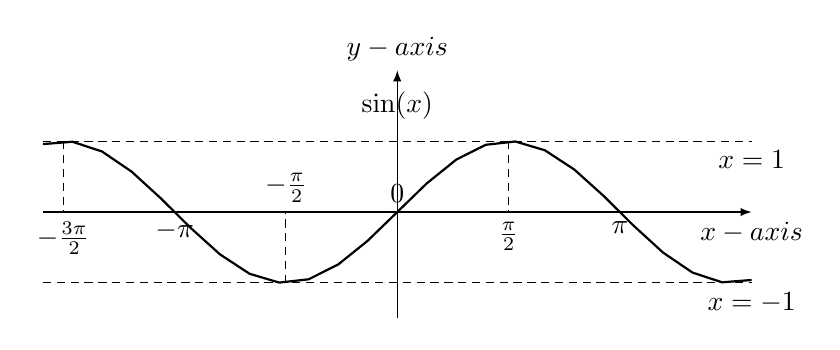
\begin{tikzpicture}[scale=0.9]
    \draw[-latex](-5,0) -- (5,0) node[below]{$x-axis$};
    \draw[-latex](0,-1.5) -- (0,2) node[above]{$y-axis$};
    \draw[black, thick, domain=-5:5] plot (\x,{sin(\x r)}) node at (0,1.5){$\sin(x)$};
    \draw [black, densely dashed](-5,1) -- (5,1) node[below]{$x=1$};
    \draw [black, densely dashed](-5,-1) -- (5,-1) node[below]{$x=-1$};
    \draw [black, densely dashed](-pi/2*3,1) -- (-pi/2*3,0) node[below]{$-\frac{3\pi}{2}$};
    \draw [black, densely dashed](-pi,0) -- (-pi,0) node[below]{$-\pi$};
    \draw [black, densely dashed](-pi/2,-1) -- (-pi/2,0) node[above]{$-\frac{\pi}{2}$};
    \draw [black, densely dashed](0,0) -- (0,0) node[above]{$0$};
    \draw [black, densely dashed](pi/2,1) -- (pi/2,0) node[below]{$\frac{\pi}{2}$};
    \draw [black, densely dashed](pi,0) -- (pi,0) node[below]{$\pi$};
\end{tikzpicture}

余弦函数:

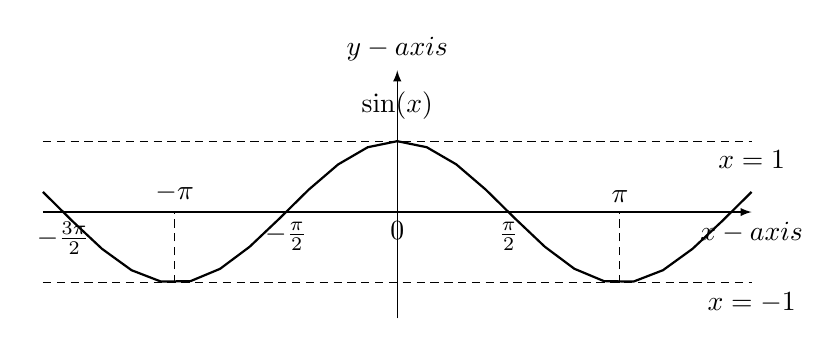
\begin{tikzpicture}[scale=0.9]
    \draw[-latex](-5,0) -- (5,0) node[below]{$x-axis$};
    \draw[-latex](0,-1.5) -- (0,2) node[above]{$y-axis$};
    \draw[black, thick, domain=-5:5] plot (\x,{cos(\x r)}) node at (0,1.5){$\sin(x)$};
    \draw [black, densely dashed](-5,1) -- (5,1) node[below]{$x=1$};
    \draw [black, densely dashed](-5,-1) -- (5,-1) node[below]{$x=-1$};
    \draw [black, densely dashed](-pi/2*3,0) -- (-pi/2*3,0) node[below]{$-\frac{3\pi}{2}$};
    \draw [black, densely dashed](-pi,-1) -- (-pi,0) node[above]{$-\pi$};
    \draw [black, densely dashed](-pi/2,0) -- (-pi/2,0) node[below]{$-\frac{\pi}{2}$};
    \draw [black, densely dashed](0,1) -- (0,0) node[below]{$0$};
    \draw [black, densely dashed](pi/2,0) -- (pi/2,0) node[below]{$\frac{\pi}{2}$};
    \draw [black, densely dashed](pi,-1) -- (pi,0) node[above]{$\pi$};
\end{tikzpicture}

\subparagraph{反三角函数} \leavevmode \bigskip

反正弦函数:

\begin{tikzpicture}
    \draw[-latex](-1.5,0) -- (1.5,0) node[below]{$x-axis$};
    \draw[-latex](0,-2) -- (0,2) node[above]{$y-axis$};
    % \draw[black, thick, domain=-1:1] plot (\x,{arcsin(\x r)}) node at (1,pi/2){$\arcsin(x)$};
    \draw[domain=-1:1,smooth,variable=\y] plot ({rad(asin(\y))},\y) node[right] {$x = \arcsin y$};
\end{tikzpicture}

\paragraph{分段函数}
\subsubsection{图像变换}
\paragraph{平移变换}
\paragraph{对称变换}
\paragraph{伸缩变换}
\subsection{极坐标系图像}
\subsubsection{描点法}
\paragraph{心形线(外摆线)}
\paragraph{玫瑰线}
\paragraph{阿基米德螺线}
\paragraph{伯努利双扭线}
\subsubsection{直角坐标系下画极坐标图像}
\subsection{参数法}
\subsubsection{摆线(平摆线)}
\subsubsection{星形线(内摆线)}
\section{常用基础知识}
\subsection{数列}
\subsection{三角函数}
\subsection{指数运算法则}
\subsection{对数运算法则}
\subsection{一元二次方程基础}
\subsection{因式分解公式}
\subsection{阶乘与双阶乘}
\subsection{常用不等式}
\end{document}
